\documentclass[11pt,]{article}
\usepackage[left=1in,top=1in,right=1in,bottom=1in]{geometry}
\newcommand*{\authorfont}{\fontfamily{phv}\selectfont}
\usepackage[]{mathpazo}


  \usepackage[T1]{fontenc}
  \usepackage[utf8]{inputenc}



\usepackage{abstract}
\renewcommand{\abstractname}{}    % clear the title
\renewcommand{\absnamepos}{empty} % originally center

\renewenvironment{abstract}
 {{%
    \setlength{\leftmargin}{0mm}
    \setlength{\rightmargin}{\leftmargin}%
  }%
  \relax}
 {\endlist}

\makeatletter
\def\@maketitle{%
  \newpage
%  \null
%  \vskip 2em%
%  \begin{center}%
  \let \footnote \thanks
    {\fontsize{18}{20}\selectfont\raggedright  \setlength{\parindent}{0pt} \@title \par}%
}
%\fi
\makeatother




\setcounter{secnumdepth}{0}

\usepackage{longtable,booktabs}

\usepackage{graphicx,grffile}
\makeatletter
\def\maxwidth{\ifdim\Gin@nat@width>\linewidth\linewidth\else\Gin@nat@width\fi}
\def\maxheight{\ifdim\Gin@nat@height>\textheight\textheight\else\Gin@nat@height\fi}
\makeatother
% Scale images if necessary, so that they will not overflow the page
% margins by default, and it is still possible to overwrite the defaults
% using explicit options in \includegraphics[width, height, ...]{}
\setkeys{Gin}{width=\maxwidth,height=\maxheight,keepaspectratio}

\title{\textbf{The effect of \emph{Ascophyllum nodosum} extracts on tomato and
pepper plant productivity and their associated fungal and bacterial
communities.}  }



\author{\Large Sébastien Renaut\textsuperscript{1,2},Jacynthe
Masse\textsuperscript{1,2}, Mengxuan Kong\textsuperscript{1,2}, Mohamed
Hijri\textsuperscript{1,2}\vspace{0.05in} \newline\normalsize\emph{\textsuperscript{1}Département de Sciences Biologiques, Institut de
Recherche en Biologie Végétale, Université de Montréal, 4101 Sherbrooke
Est, Montreal, H1X 2B2, Quebec, Canada. \textsuperscript{2}Quebec Centre
for Biodiversity Science, Montreal, Quebec, Canada}  }


\date{}

\usepackage{titlesec}

\titleformat*{\section}{\normalsize\bfseries}
\titleformat*{\subsection}{\normalsize\itshape}
\titleformat*{\subsubsection}{\normalsize\itshape}
\titleformat*{\paragraph}{\normalsize\itshape}
\titleformat*{\subparagraph}{\normalsize\itshape}





\newtheorem{hypothesis}{Hypothesis}
\usepackage{setspace}

\makeatletter
\@ifpackageloaded{hyperref}{}{%
\ifxetex
  \PassOptionsToPackage{hyphens}{url}\usepackage[setpagesize=false, % page size defined by xetex
              unicode=false, % unicode breaks when used with xetex
              xetex]{hyperref}
\else
  \PassOptionsToPackage{hyphens}{url}\usepackage[unicode=true]{hyperref}
\fi
}

\@ifpackageloaded{color}{
    \PassOptionsToPackage{usenames,dvipsnames}{color}
}{%
    \usepackage[usenames,dvipsnames]{color}
}
\makeatother
\hypersetup{breaklinks=true,
            bookmarks=true,
            pdfauthor={Sébastien Renaut\textsuperscript{1,2},Jacynthe
Masse\textsuperscript{1,2}, Mengxuan Kong\textsuperscript{1,2}, Mohamed
Hijri\textsuperscript{1,2} (\textsuperscript{1}Département de Sciences Biologiques, Institut de
Recherche en Biologie Végétale, Université de Montréal, 4101 Sherbrooke
Est, Montreal, H1X 2B2, Quebec, Canada. \textsuperscript{2}Quebec Centre
for Biodiversity Science, Montreal, Quebec, Canada)},
             pdfkeywords = {Stella Marris, 16S, ITS, microbial diversity, Illumina MiSeq},  
            pdftitle={\textbf{The effect of \emph{Ascophyllum nodosum} extracts on tomato and
pepper plant productivity and their associated fungal and bacterial
communities.}},
            colorlinks=true,
            citecolor=blue,
            urlcolor=blue,
            linkcolor=magenta,
            pdfborder={0 0 0}}
\urlstyle{same}  % don't use monospace font for urls

% set default figure placement to htbp
\makeatletter
\def\fps@figure{htbp}
\makeatother

\usepackage[left]{lineno}
\linenumbers


% add tightlist ----------
\providecommand{\tightlist}{%
\setlength{\itemsep}{0pt}\setlength{\parskip}{0pt}}

\begin{document}
	
% \pagenumbering{arabic}% resets `page` counter to 1 
%
% \maketitle

{% \usefont{T1}{pnc}{m}{n}
\setlength{\parindent}{0pt}
\thispagestyle{plain}
{\fontsize{18}{20}\selectfont\raggedright 
\maketitle  % title \par  

}

{
   \vskip 13.5pt\relax \normalsize\fontsize{11}{12} 
\textbf{\authorfont Sébastien Renaut\textsuperscript{1,2},Jacynthe
Masse\textsuperscript{1,2}, Mengxuan Kong\textsuperscript{1,2}, Mohamed
Hijri\textsuperscript{1,2}} \hskip 15pt \emph{\small \textsuperscript{1}Département de Sciences Biologiques, Institut de
Recherche en Biologie Végétale, Université de Montréal, 4101 Sherbrooke
Est, Montreal, H1X 2B2, Quebec, Canada. \textsuperscript{2}Quebec Centre
for Biodiversity Science, Montreal, Quebec, Canada}   

}

}








\begin{abstract}

    \hbox{\vrule height .2pt width 39.14pc}

    \vskip 8.5pt % \small 

\noindent The abstract will be written here


\vskip 8.5pt \noindent \emph{Keywords}: Stella Marris, 16S, ITS, microbial diversity, Illumina MiSeq \par

    \hbox{\vrule height .2pt width 39.14pc}



\end{abstract}


\vskip 6.5pt


\noindent \doublespacing \newpage 

\section{INTRODUCTION}\label{introduction}

Liquid extracts of marine macroalga are used as biostimulants in
agriculture. These extracts contain phytohormones that can influence
physiological processes even at very low concentrations Craigie (2011).
Stella Maris® is derived from fresh \emph{Ascophyllum nodosum} algae
harvested from the nutrient-laden waters of the North Atlantic off the
Eastern Coast of Canada.\\
\hspace*{0.333em}\\
The aim of this project was to develop a better understanding of the
effects of \emph{A. nodosum} extracts on plant growth. We tested the
effect of these extract on two commonly used plants (Tomato -
\emph{Solanum lycopersicum} and Pepper - \emph{Capsicum annuum}) using
different measures of productivity. In addition, we tested how the
bacterial and fungal communities responded to the addition of \emph{A.
nodosum} extracts.\\
\hspace*{0.333em} ~

\section{MATERIAL AND METHOD}\label{material-and-method}

\emph{Study design}\\
Two greenhouse experiment were set up in large trays (60x30x18 cm) in
November (tomato {[}cv: Totem Hybrid\#A371, William Dam Seeds Ltd{]})
and December (Pepper {[}cv: Ace Hybrid\#318, William Dam Seeds Ltd{]})
2015. Soil was collected from an agricultural field under organic regime
at the IRDA research station in St-Bruno (Qc, Canada) on October
7\textsuperscript{th} 2015 (loamy sand soil, 15 cm top layer collected).
Soil characteristics (pH, conductivity, nutrients, see Supplementary
Table 1) were measured by AgriDirect (Longueuil, Qc, Canada).\\
\hspace*{0.333em}\\
For each species tested (Tomato - \emph{Solanum lycopersicum}, Pepper -
\emph{Capsicum annuum}), a randomized split block design (Figure 1) was
used with four trays set up per block (eight blocks). Half of the trays
were fertilized (fertilization treatment), as described below. Half of
the trays were also planted with four replicate plants each, while the
other trays were left bare. This allowed a direct comparison of the
fungal and bacteria soil communities with respect to the fertilization
and planting treatment. ~\\
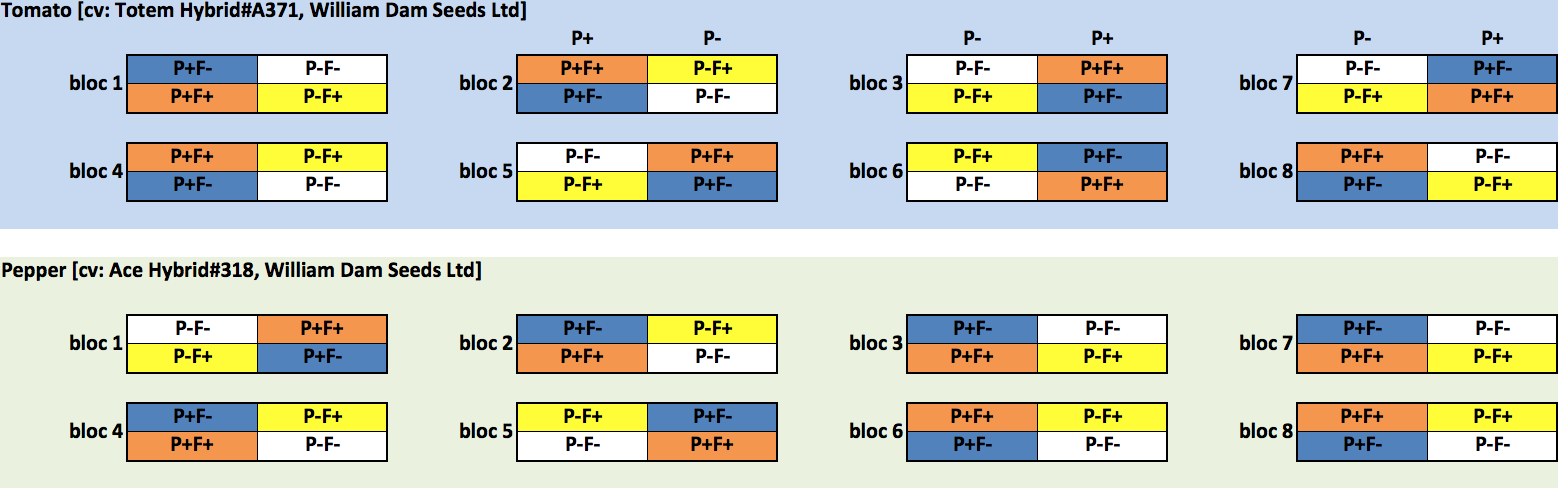
\includegraphics[width=6.25000in]{../figures/Figure1.png}\\
\textbf{Figure 1: experimental design}\\
\hspace*{0.333em}\\
Half of the tomato plants were fertilized using multipurpose organic
fertilizer (pure hen manure, 18 g per tray repeated every 4 weeks,
5-3-2) from Acti-sol (Notre-Dame-du-Bon-Conseil, Qc, Canada) in addition
to Stella Maris® (3.5 ml per 1L, each tray received 250 ml, repeated
every 2 weeks) for the duration of the experiment. The other half were
unfertilized. Stella Maris® is a registered trademark from Acadian
Seaplants Ltd. (Darmouth, NS, Canada). It is primarily composed of
\emph{Ascophyllum nodosum} seaweed and is advertized as a natural
activator of the crops' own growth and defense mechanisms to improve
root growth and resist temperature, drought, and salinity stress in
order to maximize yield and crop qualities (Acadian Seaplants Ltd.
2018). Half of the pepper plants were treated using solely Stella Maris
(3.5 ml per 1L, each tray received 250 ml, repeated every 2 weeks) for
the duration of the experiment. The other half were untreated. ~\\
Thrips were managed with \emph{Neoseiulus cucumeris} (syn.
\emph{Amblyseius cucumeris}) (100 bags), Fungus gnat and thrips were
also controlled using predatory mite \emph{Gaeolaelaps gillespiei} (1L).
Plants were treated once a week with Oïdium Milstop to control the
fungus.\\
\hspace*{0.333em}\\
\hspace*{0.333em}\\
\emph{Plant productivity}\\
At the end of the experiment, plant productivity was assessed by
measuring four different traits (fruit number, average fruit weight,
shoots fresh weight, roots fresh weight) on three plants chosen randomly
per tray (for each treatment {[}fertilization/control{]}, species
{[}tomato/pepper{]} and block {[}eight blocks{]}) for a total of 96
samples. In addition, both shoots and roots were dried in a 70 degrees
drying oven, and dry weights were measured after 48 hours. Together,
these traits are expected to represent well the plant overall
productivity.\\
\hspace*{0.333em}\\
\hspace*{0.333em}\\
\emph{Sample preparation, DNA extraction and High throughput
sequencing}\\
We sampled both the microbial and fungal communities from soil and root
samples. Soil DNA was extracted using XXX DNA isolation kit with YYY g
of soil. Roots were first washed with sterile water and DNA was
extracted using XXX DNA isolation kit with YYY g of root samples.
Amplicon sequencing targeting 16S rRNA gene (bacteria) and ITS (fungi)
was performed on both root and soil samples.\\
\hspace*{0.333em}\\
In order to target fungi, we used fungal primers ITS3\_KYO2
(5'-ACACTGACGA CATGGTTCT ACAGATGAAGAAC GYAGYRAA-3') and ITS4\_KYO3
(5'-TACGGT AGCAGAGACTT GGTCTCTBTTV CCKCTTCACTCG-3') to produce a final
amplicon size of \textasciitilde{}430bp. This primer pair should target
the Internal transcribed spacer and inhibit the amplification of plant
sequences and enable the selective amplification of fungal communities
from soil, mycorrhizal and other environmental samples (Toju \emph{et
al.} 2012).\\
\hspace*{0.333em}\\
Bacterial primers 341F (5'-CCTACGGG NGGCWGCAG-3') and 805R (5'-GACTACC
AGGGTATC TAATC-3') producing a final amplicon size of
\textasciitilde{}464b and targeting specifically the bacterial V3-V4
region of the 16S ribosomal gene were chosen given that they has been
used extensively in high-throughput sequencing studies in a range of
environments Toju et al. (2012). This primer pair was shown to be the
least biased among 512 primer pairs evaluated in silico for bacterial
amplification Klindworth et al. (2013).\\
\hspace*{0.333em}\\
DNA samples were then barcoded, pooled and sequenced (2X300bp,
paired-end) using an Illumina MiSeq (San Diego, CA, USA) sequencer at
the Genome Quebec Innovation Centre (Montreal, Canada). Sequences were
demultiplexed by the sequencing facility (Genome Quebec Innovation
Centre) and further processed as described below.\\
\hspace*{0.333em}\\
\hspace*{0.333em}\\
\emph{Bioinformatics}\\
All bioinformatics, statistical, and graphical analyses further
described were performed in R 3.4.4 (R Core Team 2018) and detailed
scripts are available here
(\url{https://github.com/seb951/Acadian_Seaplants}).\\
\hspace*{0.333em}\\
We used the \texttt{R} package \texttt{dada2} Callahan et al. (2016) to
infer \emph{Amplicon Sequence Variants (ASVs)}. \texttt{Dada2} offers
accurate sample inference from amplicon data with single-nucleotide
resolution in an open source (R) environments. Unlike the Operational
Taxonomic Unit (OTU) approach (e.g. Schloss et al. (2009), Caporaso et
al. (2010)), ASV are not treated as cluster of sequences defined with an
\emph{ad hoc} sequence similarity threshold, thus allowing sequences and
abundance counts to be compared among studies Callahan et al. (2016).\\
\hspace*{0.333em}\\
First, sequences were trimmed following strict quality thresholds (see
parameter details in the accompanying \texttt{R} scripts). Following
this, we applied the error model algorithm of \texttt{dada2} which
incorporates quality information after filtering, unlike other OTU based
methods. Then dereplication, sample inference, merging of paired end
reads and removal of chimera reads were performed in order to obtain a
sequence (ASVs) table of abundance per sample. Taxonomy was also
assigned using the Ribosomal Database Project (RDP) Naive Bayesian
Classifier algorithm from Wang et al. (2007). Depending on support
(minimum bootstrap support of 80), we assigned taxonomy from Kingdom to
species. We used the silva database formatted for \texttt{dada2} to
infer bacterial taxa Callahan (2018). We used the Community (2018) fasta
release (including singletons) to infer fungal taxa after formatting it
to the \texttt{dada2} format using a custom \texttt{R} script. The
pipeline was run on a multithreaded (48 CPUs) computer infrastructure
provided by Westgrid
(\url{https://www.westgrid.ca/support/systems/cedar}) and Compute Canada
(www.computecanada.ca). Note that the pipeline was run separately for
fungal-root, fungal-soil, bacteria-soil and bacteria-root samples given
the markedly different type of amplicons, taxa and error models of each
dataset. ~\\
\hspace*{0.333em}\\
\emph{Statistical analyses - plant productivity}\\
We tested for the effect of species (tomato vs pepper), fertilization
and their interaction on six plant productivity measures (fruit number,
average fruit weight, shoots fresh weight, roots fresh weight, shoots
dry weight, roots dry weight). We used linear mixed effect models (LMM)
in the R package \texttt{nlme} Pinheiro et al. (2017), which are more
appropriate than an Analysis of Variance (ANOVA) given the current block
design (blocks and replicates nested within a block were treated as
random variables). All six plant productivity measures were either
square root or log transformed in order to help satisfy the assumption
of normality of the residuals in the LMM statistical framework. For the
variables \emph{fruit number} and \emph{average fruit weight}, we also
used a permutation-based 2-way ANOVA (Anderson \& Legendre (1999)) given
that the residuals of the LMM were not normally distributed, and results
were similar.\\
\hspace*{0.333em}\\
\hspace*{0.333em}\\
\emph{Statistical analyses - microbial and fungal diversity}\\
We analysed separately fungal-root, fungal-soil, bacterial-root and
bacterial-soil ASV diversity. For each of these four datasets, we
removed samples that showed poor sequencing output and contained few
ASVs. In order to do this, we summed the abundance of all ASVs for each
sample (\(\sum_{i=1}^n ASV\)) and eliminated samples that had fewer that
the mean sum (\(\overline{\sum_{i=1}^n ASV}\)) - 4\(\sigma\) (four
standard deviations). In addition, we removed ASVs from our dataset that
were present in fewer than 5\% of the samples (less than ten individuals
in the soil samples, and less than five in the root samples). This was
done to remove very rare ASVs which were unique to a block or replicate,
but not found in the majority of a treatment.\\
\hspace*{0.333em}\\
We then conducted community-based analyses looking at the effect of the
fertilization treatment on the abundance ASV taxa in the tomato and
pepper experiments. To reduce the complexity of the datasets, relative
abundance of all taxa were calculated per family using the \texttt{R}
package \texttt{dplyr} Wickham et al. (2015). Barplots were drawn using
\texttt{ggplot2} Wickham (2016) to vizualize communities. ASV
(\(a\))-diversity was calculated for each sample using the inverse
Simpson diversity index in \texttt{vegan} Oksanen et al. (2013). The
effect of fertilization treatment, species (and planting for soil
communities) were assessed using a linear mixed-effect (LMM) model in
the R package \texttt{nlme} Pinheiro et al. (2017), given the
unbalanced, replicated block design. Alpha diversity was log transformed
in order to help satisfy the assumption of normality of the residuals of
the LMM statistical framework.\\
\hspace*{0.333em}\\
Using the community matrix data of ASVs abundance, we performed
PERmutational Multivariate ANalysis Of VAriance tests (PERMANOVA;
Anderson (2001)) to identify relationships between the communities
according to the experimental design. ASV abundance data was
Hellinger-transformed and significance was assessed using 10,000
permutations in \texttt{vegan} Oksanen et al. (2013). Blocks and
replicates nested within blocks were factored as strata (blocks) in the
model.\\
\hspace*{0.333em}\\
We also performed constrained ordinations (CCAs) using
Hellinger-transformed ASV abundance data in \texttt{vegan} Oksanen et
al. (2013) to visually assess (\emph{species} scaling based on ASV
matrix) the grouping of samples, ASVs and their association with
productivity variables. Data were analysed separately for fungal-root,
fungal-soil, bacterial-root and bacterial-soil, but also according to
species (tomato/pepper), given that analyses of \(a\) diversity showed
that tomato and pepper were markedly different. This gave a total of
eight CCAs. Data were constrained based on four of the productivity
measures (fruit number, average fruits weight, shoots fresh weight,
roots fresh weight). We excluded the shoot \& root dry weights as
constraints to simplify the model and given that they were highly
correlated with the fresh weigth already included as constraints
(\(r^2\)=0.98 and 0.76 for shoot dry/fresh weights and root dry/fresh
weights, respectively). ~\\
\hspace*{0.333em}\\
Finally, we attempted to identify candidate ASVs positively associated
with productivity. As such, we identified the ten ASVs most positively
associated with the measures of fruit number, shoots fresh weight and
roots fresh weight from each constrained ordinations for a total of 40
fungal and 40 bacterial candidates ASVs. We aligned candidate sequences
from these candidates ASVs using the Bioconductor \texttt{R} package
\texttt{decipher} Wright (2016) and build pairwise distances matrices
using a JC69 substitution models of DNA sequence evolution (equal base
frequencies, Jukes \& Cantor (1969)) in \texttt{phangorn} Schliep
(2010). Phylogenetic trees for bacteria and fungi were plotted using
\texttt{ape} Paradis, Claude \& Strimmer (2004). This permitted to
identify if similar candidate ASVs were found under different
experimental conditions (soil/root, pepper/tomato), thus reinforcing
their role in productivity increase, and decreasing the change that
these are false positive.\\
\hspace*{0.333em} ~

\newpage  

\section{RESULTS}\label{results}

\emph{productivity}\\
We tested the effect of the fertilization treatment on six measures of
overall plant growth and productivity (fruit number, average fruit
weight, shoots fresh weight, shoots dry weight, roots fresh weight,
roots dry weight) for both tomato and peppers. Visually, both above
ground and below ground plant structure grew larger in fertilized
plants, in addition to producing more fruits (see Figure 2 for some
examples of the striking difference between fertilized and unfertilized
plants). ~\\
\includegraphics[width=5.20833in]{../figures/productivity/Figure_2_photos_productivity.png}\\
\textbf{Figure 2: Plant productivity. Photos were taken at the end of
the experimental treatment. In each photo, fertilized plants are on the
left. A: pepper plants, B: pepper roots, C: pepper fruits and D: tomato
fruits.}\\
\hspace*{0.333em}\\
Statistically, all six productivity measures significantly differed
according to species, and five of those were significantly different
according to the fertilization treatment. The only exception was the
average fruit weight which did not differ between fertilized and control
plants (LMM, \(F_{(1,69)}\) = 1.27, \emph{p}-value=0.26). However the
model did reveal a significant interaction between treatment and plant
(\(F_{(1,69)}\) = 9.6, \emph{p}-value=0.0028). In fact, when testing
only the pepper plants, the effect of fertilization on average fruit
weight was significantly higher in the fertilized pepper plants
(\(F_{(1,23)}\) = 10.84, \emph{p}-value=0.0032).\\
\hspace*{0.333em}\\
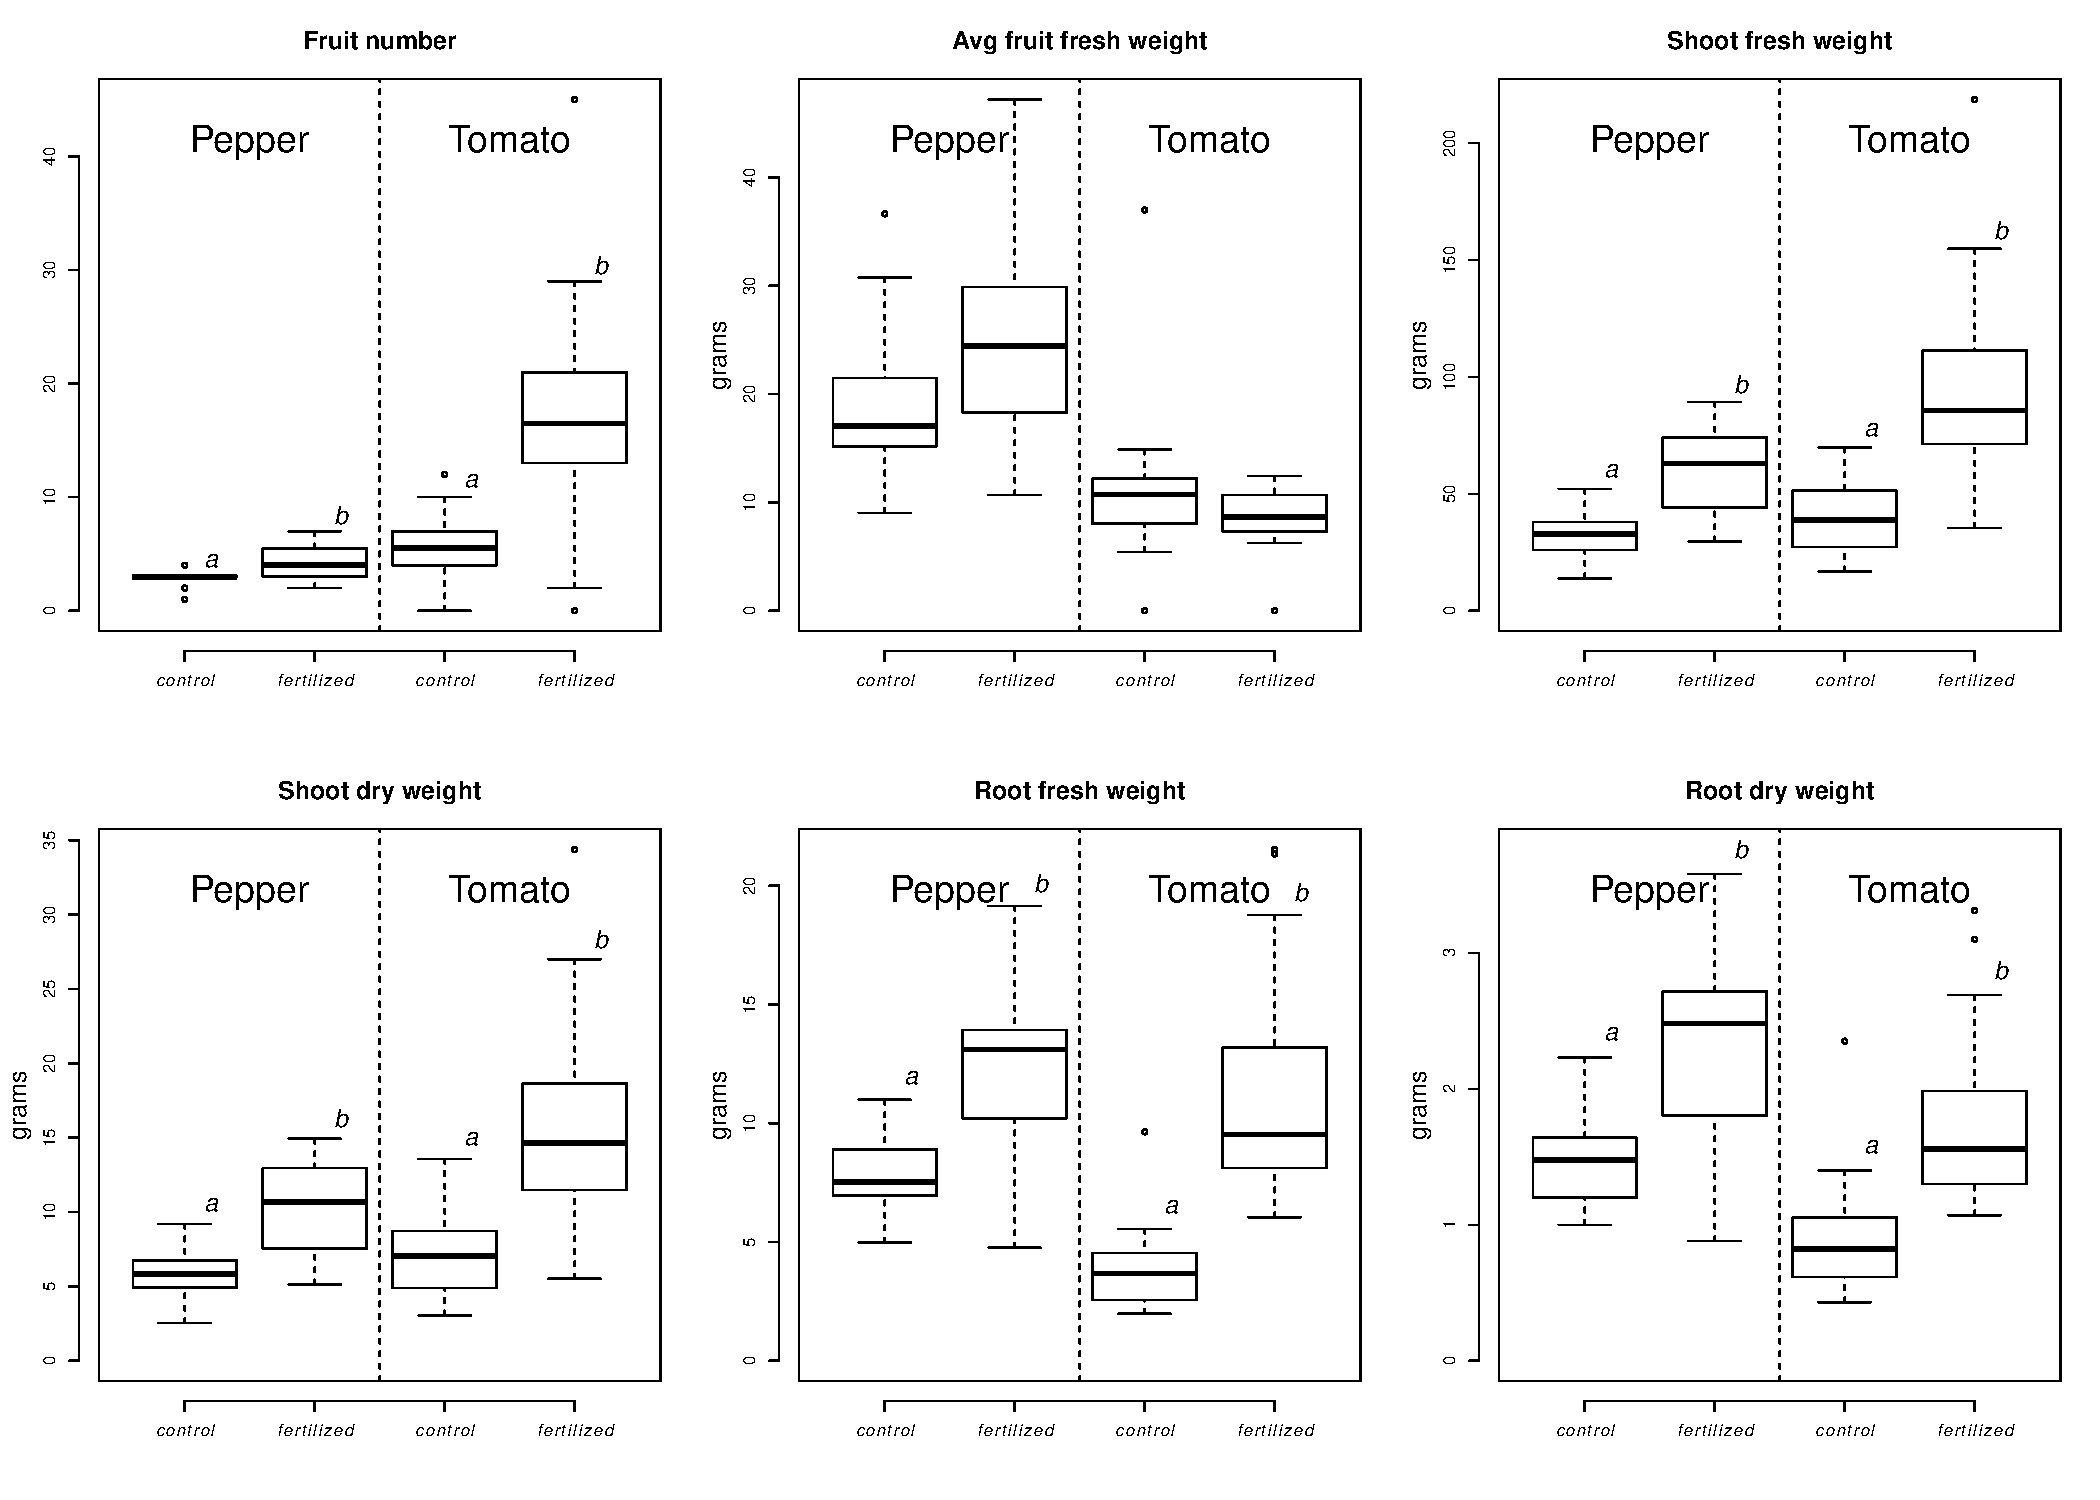
\includegraphics[width=6.25000in]{../figures/productivity/Figure_3_productivity.pdf}\\
\textbf{Figure 3: measures of plant productivity.}\\
\hspace*{0.333em}\\
\hspace*{0.333em}\\
\emph{Sequencing}\\
A total of 2.7 million paired-end raw reads were obtained for all
samples combined (976,000 for fungi-soil, 920,000 for fungi-root,
309,000 for bacteria-soil and 535,000 for bacteria-root, Table 1). Note
that sequencing samples were analysed separately for fungal-soil,
fungal-root, bacteria-soil and bacteria-root conditions. On average,
46,965 paired-end reads were obtained per sample. After quality filters
were applied, including removing chimeras, and paired-end reads were
merged, an average of 18,435 sequences remained. While 192 soil samples
for fungi and bacteria, and 92 root samples for fungi and bacteria were
sequenced, three fungi-soil samples, 13 fungi-root samples and two
bacteria-root samples were removed because they had to few reads based
on our strict quality thresholds.\\
\hspace*{0.333em}\\
The \texttt{dada2} pipeline infered, on average, 112 Amplicon Sequence
Variants per sample (average of 163 fungal-soil ASV, 49 fungal-root
ASVs, 112 bacterial-soil ASVs and 122 bacterial-root ASVs). Many of
those were unique to one of a few samples (total number of 6,178
fungal-soil, 930 fungal-root, 10,120 bacterial-soil and 3,143
bacterial-roots ASVs). After quality filtering ASVs that were found in
fewer than 10\% of the samples, we retained 418, 169, 206 and 250 ASVs
and which comprised 91\%, 88\%, 50\% and 85\% of all reads in the
fungal-soil, fungal-root, bacterial-soil and bacterial-root samples,
respectively.\\
\hspace*{0.333em}\\
\hspace*{0.333em}

\begin{longtable}[]{@{}lrrrr@{}}
\caption{Sequencing and ASV summary}\tabularnewline
\toprule
& fungi-soil & fungi-root & bacteria-soil & bacteria-root\tabularnewline
\midrule
\endfirsthead
\toprule
& fungi-soil & fungi-root & bacteria-soil & bacteria-root\tabularnewline
\midrule
\endhead
Nb\_seq\_sum & 976,000 & 309,000 & 920,000 & 535,000\tabularnewline
Nb\_seq\_mean & 51,381 & 32,208 & 47,907 & 56,365\tabularnewline
Nb\_seq\_mean\_filtered & 38,045 & 14,635 & 38,287 &
46,081\tabularnewline
Nb\_seq\_mean\_filt\_merged & 32,014 & 13,335 & 13,780 &
41,058\tabularnewline
Nb\_seq\_mean\_filt\_merg\_non\_chimeras & 24,737 & 8,505 & 12,049 &
28,451\tabularnewline
Nb\_samples & 192 & 96 & 192 & 96\tabularnewline
Nb\_samples\_trimmed & 189 & 83 & 192 & 94\tabularnewline
ASV\_sum & 6,178 & 930 & 10,120 & 3,143\tabularnewline
ASV\_sum\_trimmed & 418 & 169 & 206 & 250\tabularnewline
ASV\_persample & 163 & 49 & 112 & 122\tabularnewline
\bottomrule
\end{longtable}

~\\
\hspace*{0.333em}\\
\emph{Root \& soil microbial and bacterial diversity}\\
We then analysed the whole community structure and report the relative
abundance of taxa (family) for the fungal-soil, fungal-root,
bacteria-soil and bacteria-root conditions (Figure 4). Fungal
communities were dominated by Nectriaceae, both the in the root and soil
samples. Bacterial root communities were largely dominated by the
Cyanobacteria phylum (identified as \emph{chloroplast} according to the
Ribosomal Database Project Naive Bayesian Classifier and the silva
database). In fact, these ASVs are likely sequenced chloroplasts from
the plants themselves, despite the fact that the primer pair used should
have primarly targeted the bacterial V3-V4 region of the 16S ribosomal
gene. The bacterial family Bacilaceae dominated to a lesser extent the
soil communities.\\
\hspace*{0.333em}\\
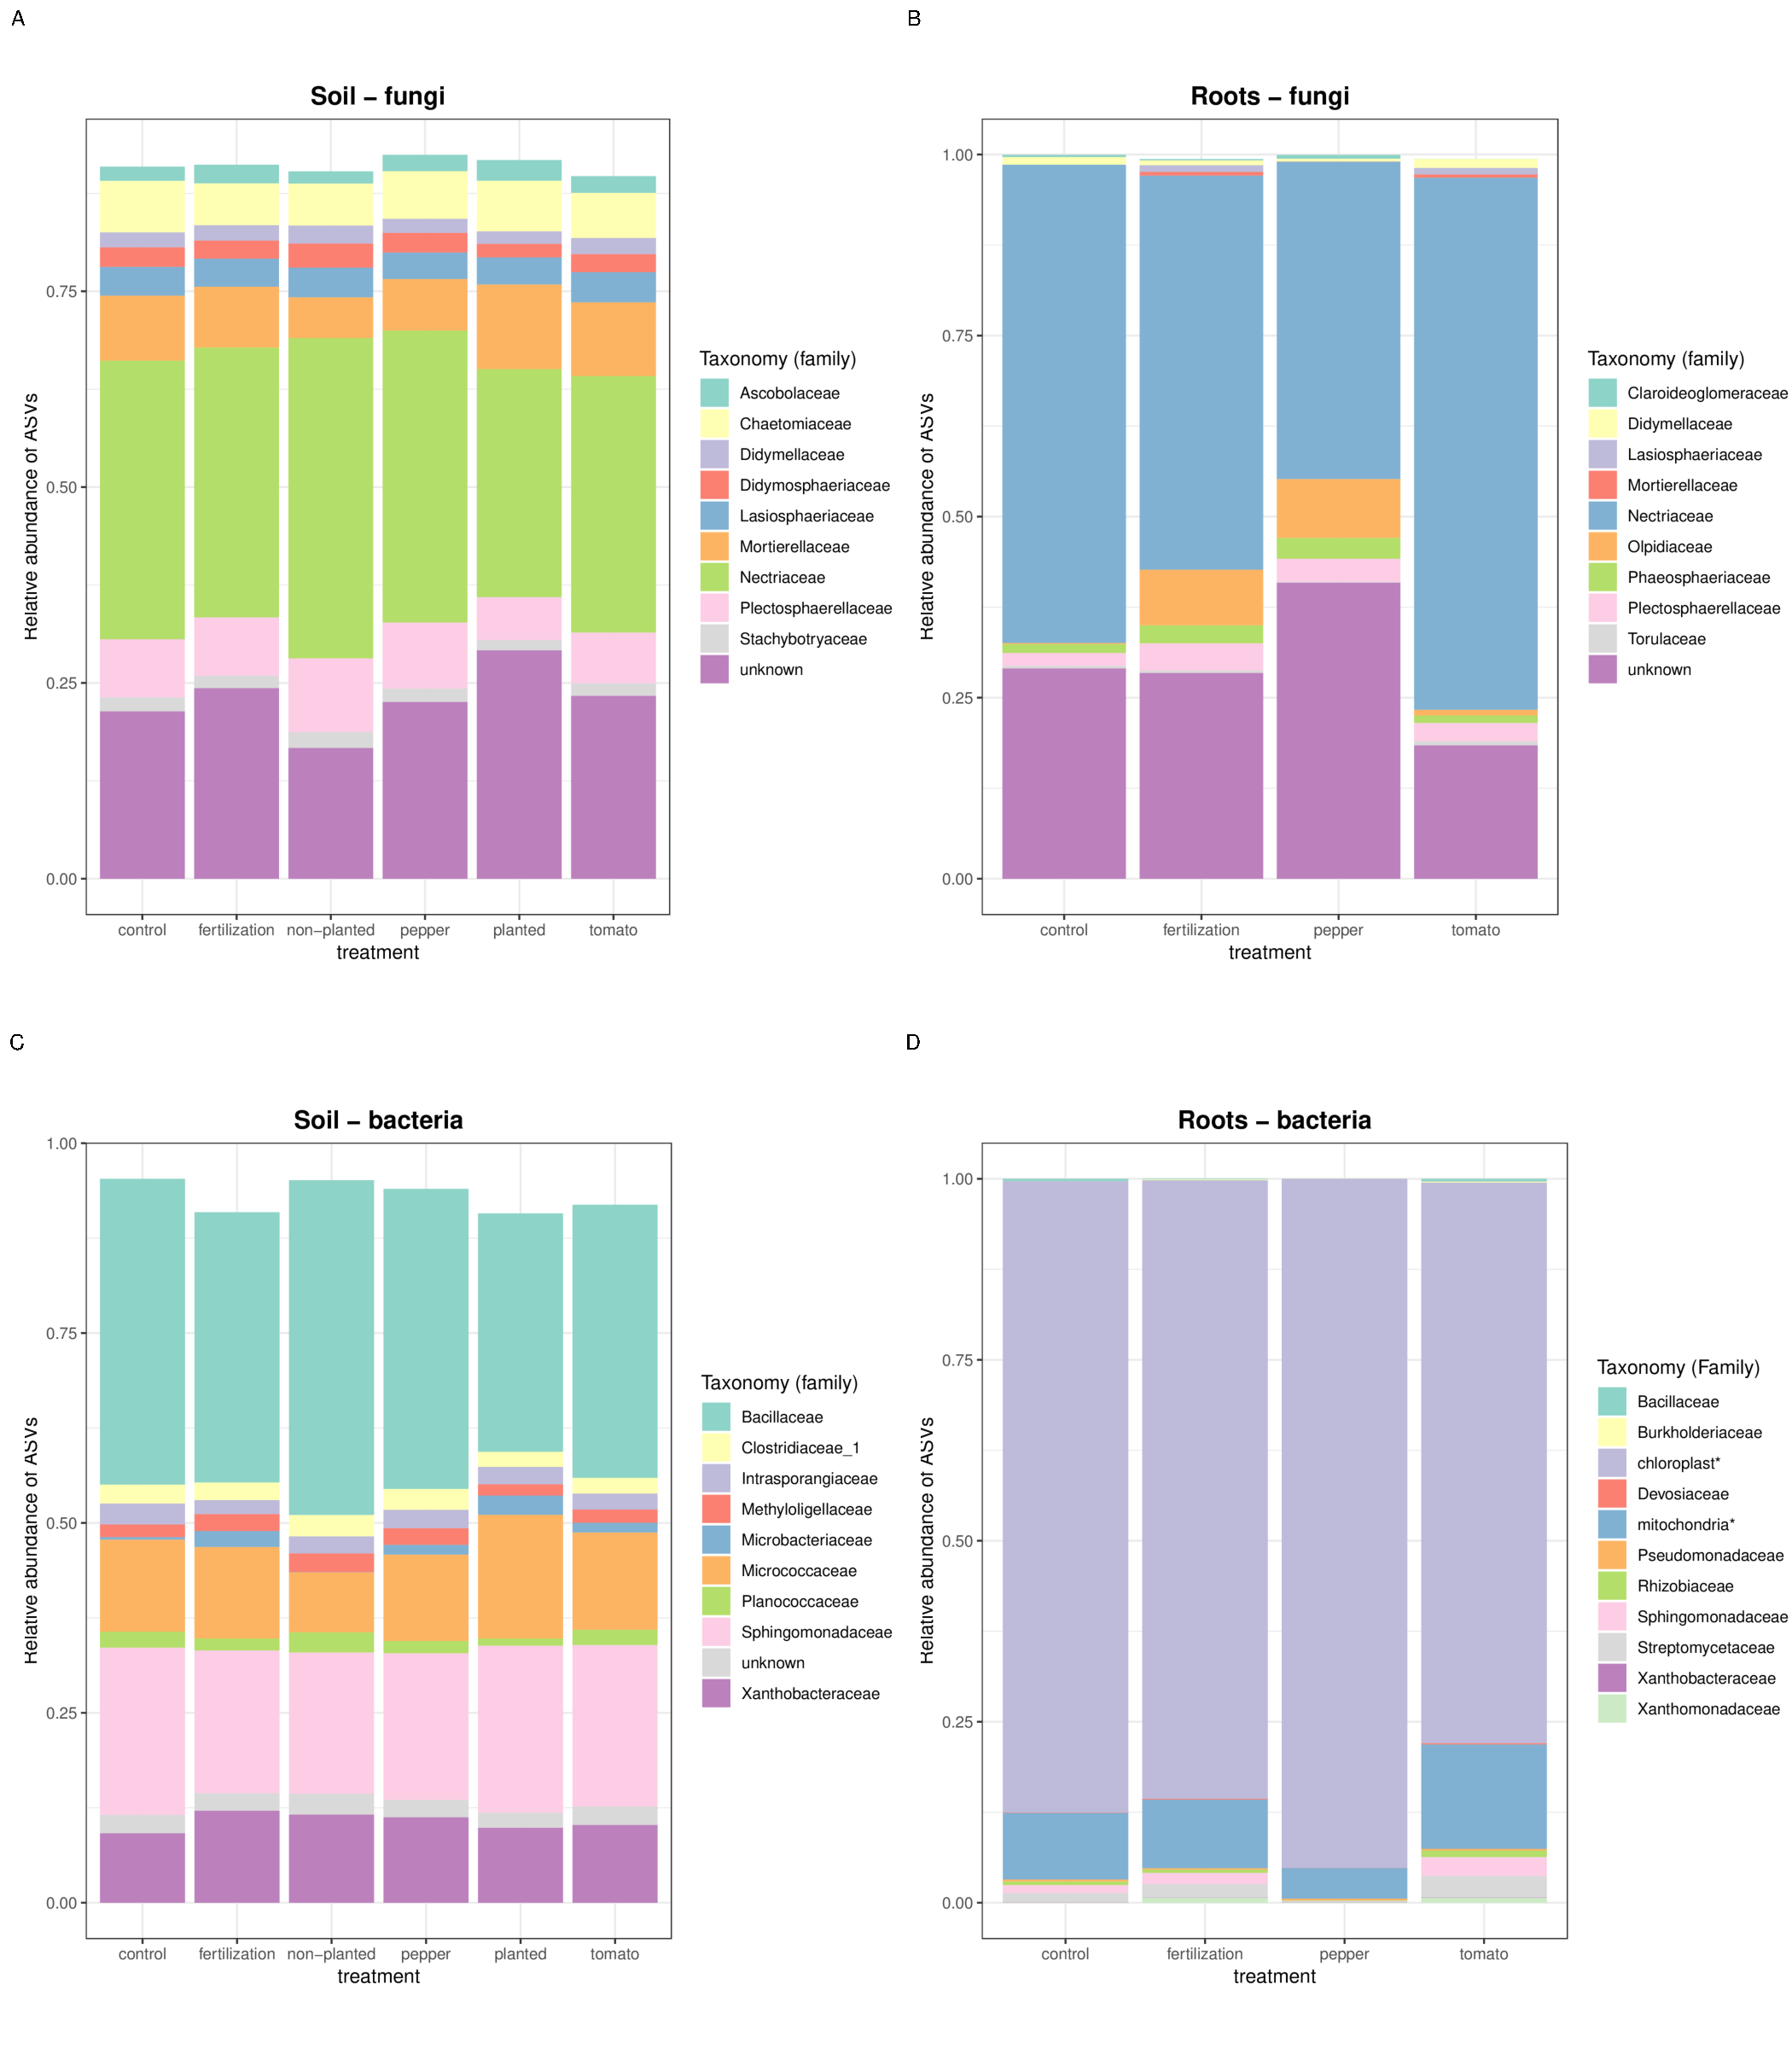
\includegraphics[width=7.29167in]{../figures/Figure4_FAMILY_barplots.pdf}\\
\textbf{Figure 4: Barplots fo the relative abundance of ASVs for
fungal-root, fungal-soil, bacteria-soil and bacteria-root}\\
\hspace*{0.333em}\\
\hspace*{0.333em}\\
\emph{Local (\(a\)-diversity)}\\
The diversity of each site (\(a\)-diversity) was calculated seperately
for each sample and under each experimental conditions (fungi-soil,
fungi-root, bacteria-soil and bacteria-root, Figure 5). Linear mixed
effects models used to assess significance. In soils samples, fungal
diversity differed with respect to the fertilization
(\(F_{(1,161)}\)=14.35, \emph{p}-value\textless{}0.0001) and planting
(\(F_{(1,161)}\)=41.00, \emph{p}-value\textless{}0.0001) treatment, but
not the species (\(F_{(1,161)}\)=0.13, \emph{p}-value=0.72). In root
samples, fungal diversity differed with respect to the fertilization
treatment (\(F_{(1,56)}\)=13.56, \emph{p}-value=0.001), and the species
tested (\(F_{(1,56)}\)=74.31, \emph{p}-value=0.003). In soil samples,
bacterial diversity differed with respect to the fertilization treatment
(\(F_{(1,165)}\)=46.25, \emph{p}-value\textless{}0.0001), planting
(\(F_{(1,165)}\)=48.77, \emph{p}-value\textless{}0.0001) and species
(\(F_{(1,165)}\)=10.22, \emph{p}-value=0.002). In root samples,
bacterial diversity differed with respect to the fertilization treatment
(\(F_{(1,67)}\)=16.48, \emph{p}-value=0.0001), and the species tested
(\(F_{(1,67)}\)=523.42, \emph{p}-value\textless{}0.0001). ~\\
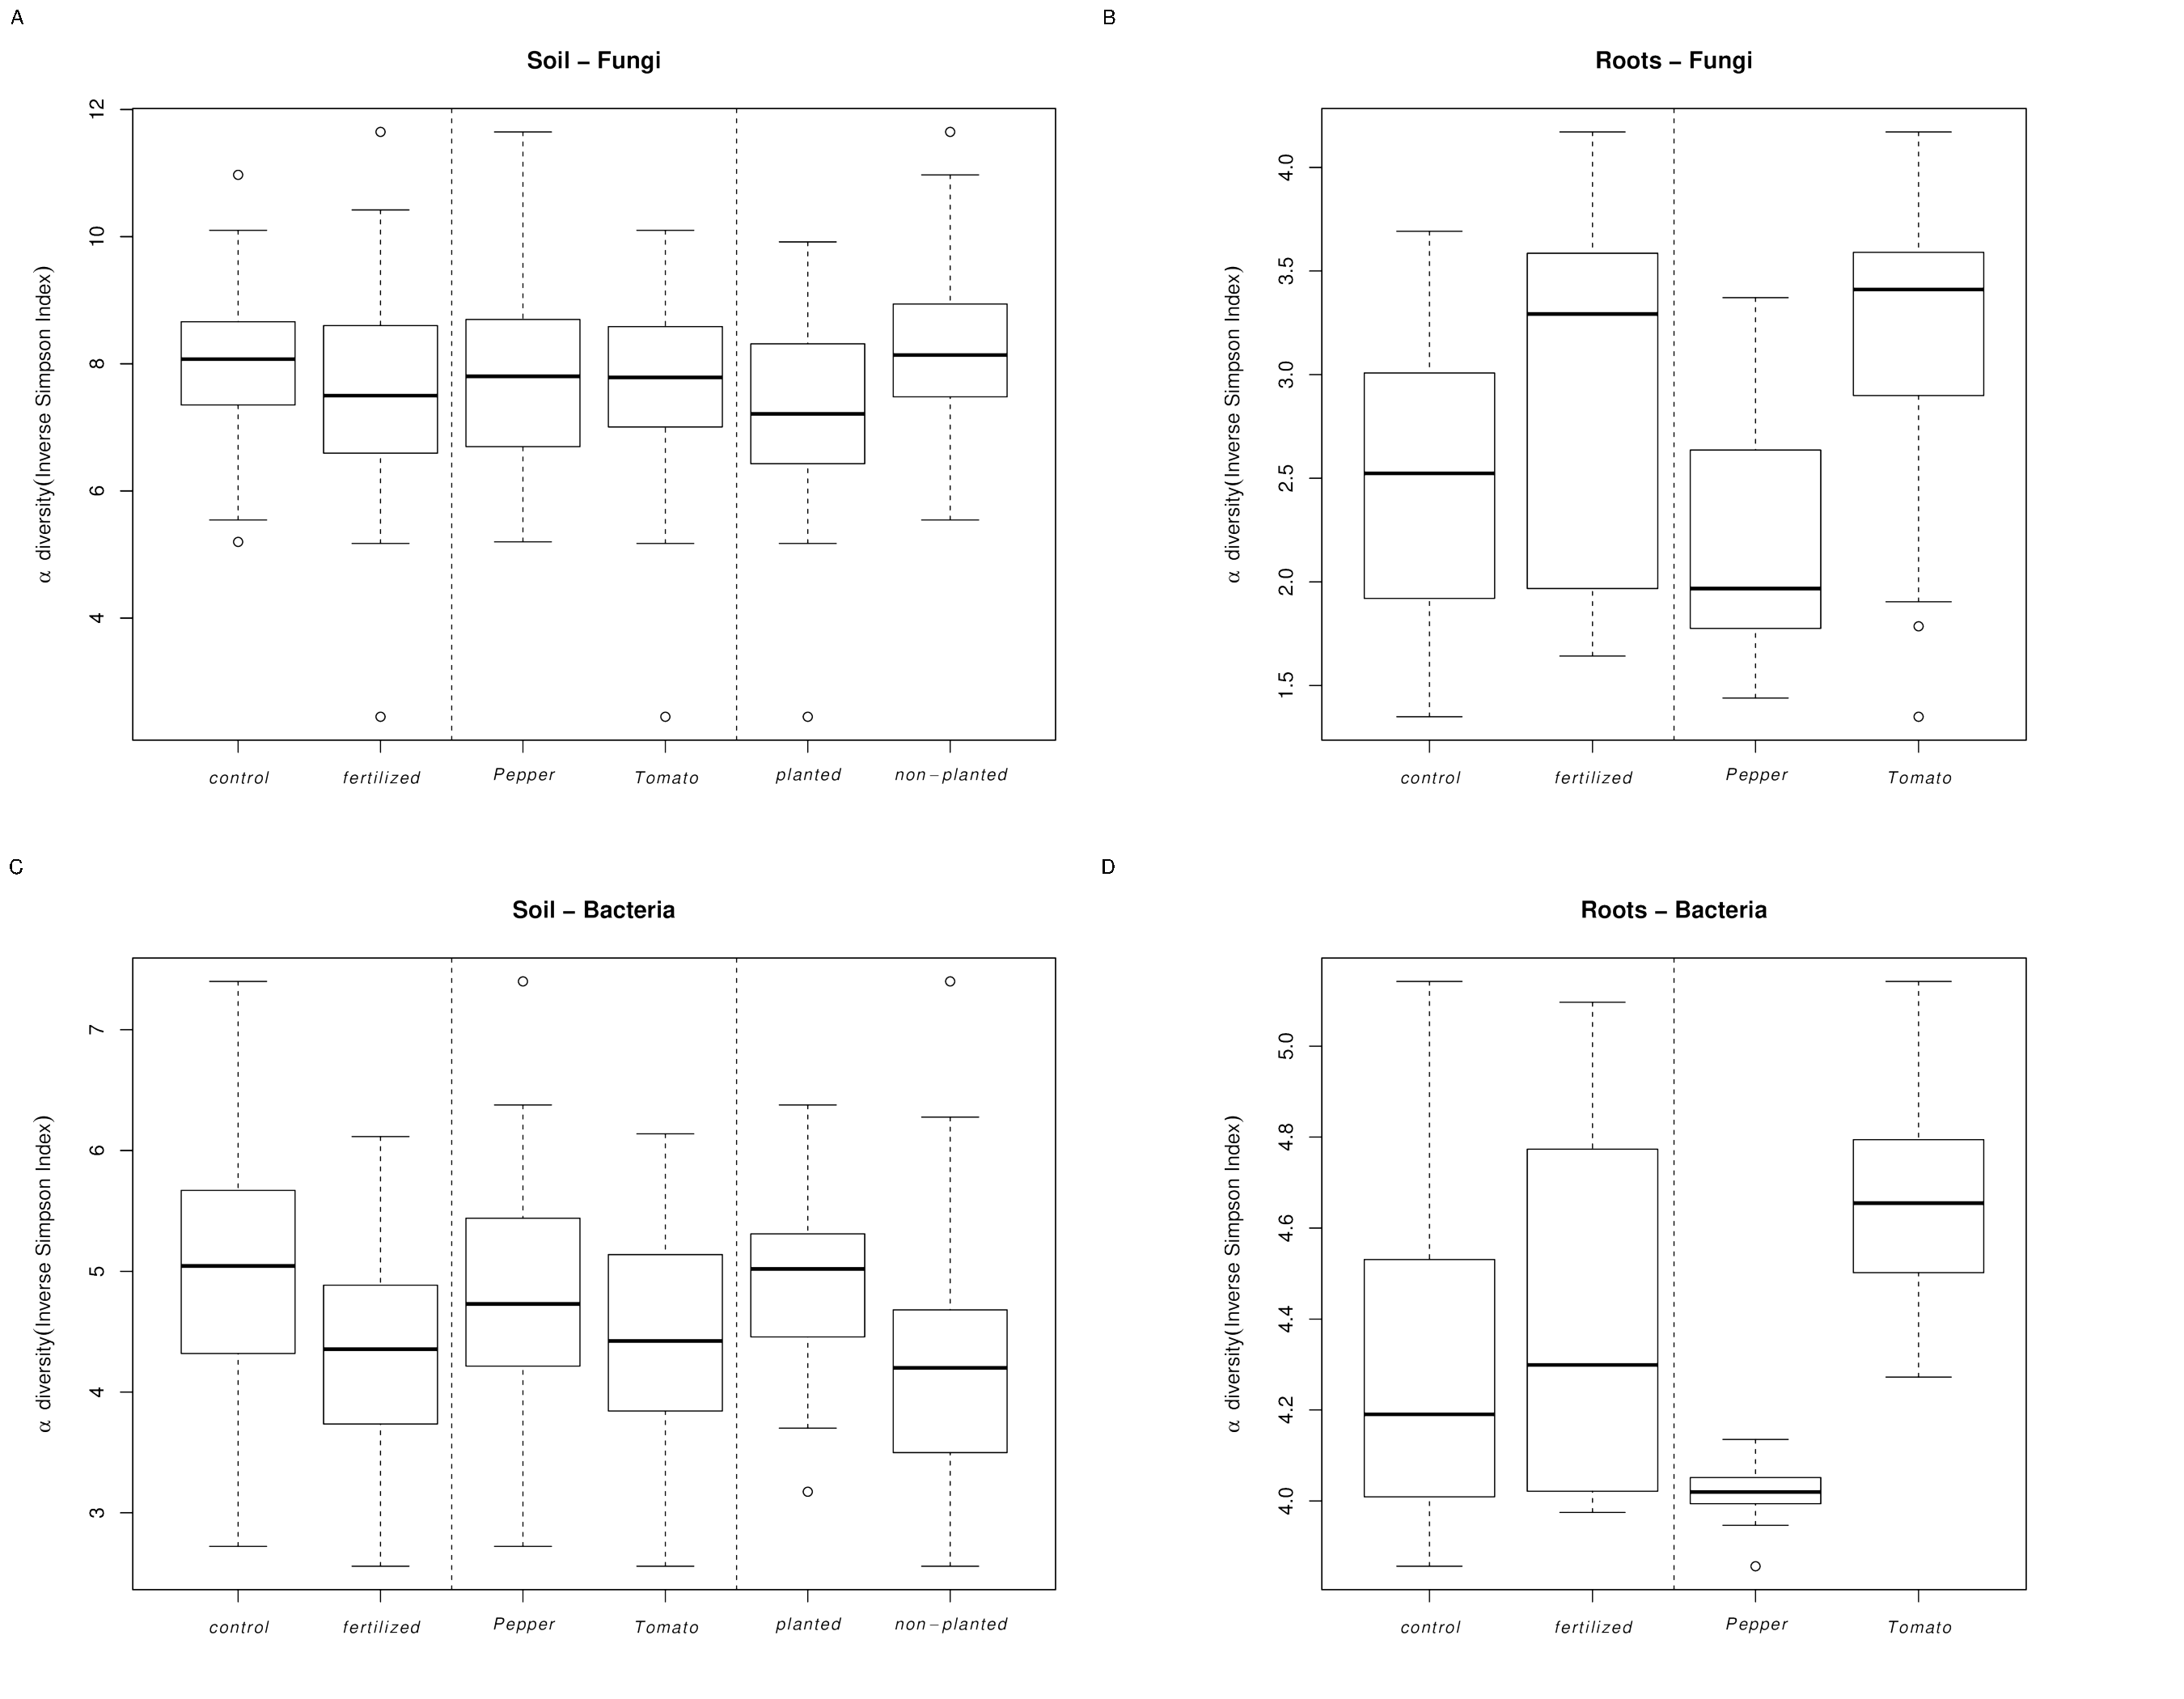
\includegraphics[width=6.25000in]{../figures/Figure5_alpha.pdf}\\
\textbf{Figure 5: Boxplot of alpha diversity according to the treatment,
species and planting effect for fungal-root, fungal-soil, bacteria-soil
and bacteria-root.}\\
\hspace*{0.333em}\\
\hspace*{0.333em}\\
\emph{Differences in species composition among sites}\\
Using a PERMANOVA statistical framework, we identified that for all
conditions, communities differed with respect to the fertilization
treatment (Table 2). Soil fungal and bacterial communities differed the
most according to whether the tray was planted (greatest \% of variance
explained, Table 2) , while root communities differed the most between
tomato and pepper plants.

\begin{longtable}[]{@{}lllll@{}}
\caption{summary of PERMANOVAs*}\tabularnewline
\toprule
& fungi-soil & fungi-root & bacteria-soil & bacteria-root\tabularnewline
\midrule
\endfirsthead
\toprule
& fungi-soil & fungi-root & bacteria-soil & bacteria-root\tabularnewline
\midrule
\endhead
fertilization & 0.02 (4e-04) & 0.04 (0.0013) & 0.03 (1e-04) & 0.01
(0.0705)\tabularnewline
planted & 0.15 (1e-04) & NA & 0.06 (1e-04) & NA\tabularnewline
species & 0.02 (2e-04) & 0.2 (1e-04) & 0.01 (0.0032) & 0.42
(1e-04)\tabularnewline
fertilization:planted & 0.01 (0.008) & NA & 0.02 (1e-04) &
NA\tabularnewline
fertilization:species & 0.01 (0.0705) & 0.03 (0.0094) & 0.01 (0.002) &
0.01 (0.0973)\tabularnewline
planted:species & 0.01 (0.1597) & NA & 0.01 (0.1767) & NA\tabularnewline
fertilization:planted:species & 0 (0.7956) & NA & 0.01 (0.1179) &
NA\tabularnewline
\bottomrule
\end{longtable}

*\(r^2\) {[}percentage of variance explained by the term in the model{]}
and associated \emph{p}-values in parentheses. ~\\
\hspace*{0.333em}\\
\emph{Constrained ordinations and candidate ASVs}\\
Constrained ordinations indicated how fertilized samples clustered
together according to their fungal or bacterial communities (Figure 6).
It also shows a similar association of three of the constrain variables
(productivity measures of root fresh weight, shoots fresh weight and
fruit number), while average fruit weight behave differentially (in fact
nearly orthogonally to the other three constrains in most
ordinations).\\
\hspace*{0.333em}\\
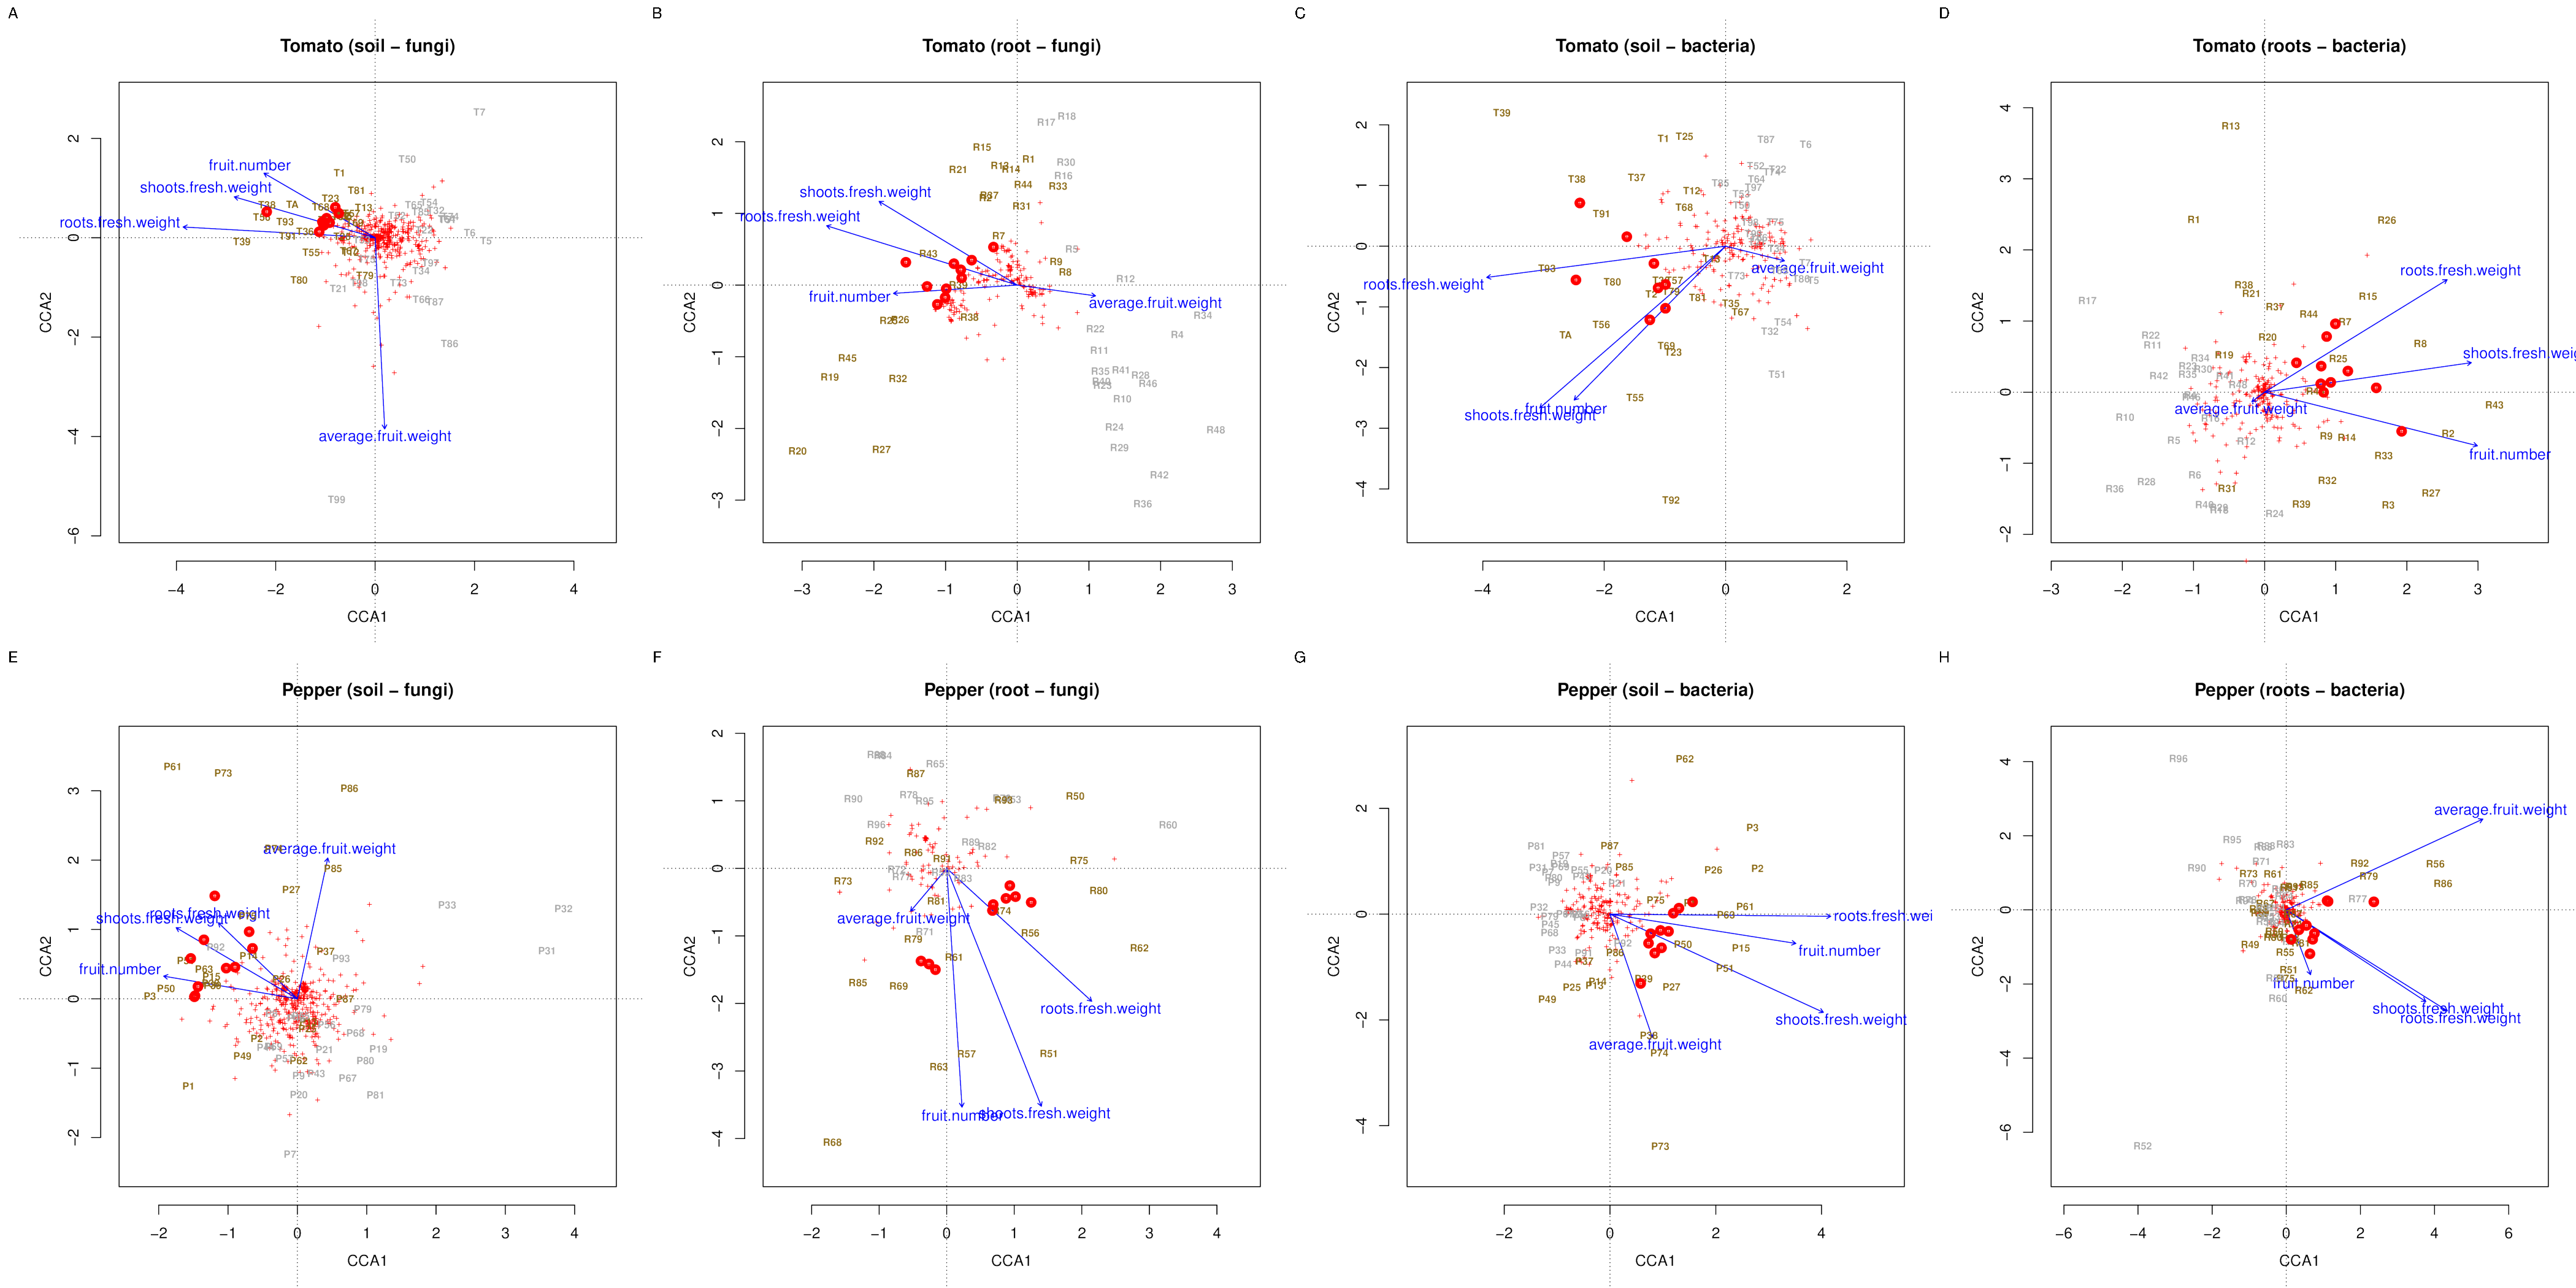
\includegraphics{../figures/Figure6_rda.pdf}\\
\textbf{Figure 6: Constrained ordinations. Samples are labelled and
colored in gray (unfertilized) or dark yellow (fertilized). Red crosses
represent individual ASVs, while red points represent the ten ASVs most
closely associated wih the three productivity measures of root fresh
weight, shoots fresh weight and fruit number. Blue arrows are the four
productivity measures used as constrains in the ordinations.}\\
\hspace*{0.333em}\\
\hspace*{0.333em}\\
Next, we identified, for each ordination, the ten ASVs most closely
related to the three constrains which behaved in a similar fashion
(productivity measures of root fresh weight, shoots fresh weight and
fruit number). These ASVs were considered as putative candidates
sequences most positively impacted (increase presence of the ASV) by
fertilization. We further analysed the corresponding sequences for these
eigthy candidates (ten candidates * eight ordinations) ASVs in two
seperate alignments (one for fungi and one for bacterial ASVs) and their
accompanying neighbouring joining trees. In fungi, we identified one
cluster of ASVs taxonomically assigned to \emph{Olpidium brassicae}
(fungal obligate parasite in the phylum Chytridiomycota) that forms the
majority of ASVs most closely related to productivity. In addition, we
identified five different ASVs in both species and both root and soil
closely related phylogenetically. Given that no taxonomy was assigned to
these sequences through the \texttt{dada2} RDP bootstrap approach, we
used a BLASTn Altschul et al. (1997) approach (against NCBI nr) to
identify the most closely related sequences. We identified this cluster
of ASVs as \emph{Rhogostoma schuessleri (BLASTn, e-value=2e-74)}, a
protist in the phylum Cercozoa, which are known to be present in the
soil and phyllosphere Dumack et al. (2017) .\\
\hspace*{0.333em}\\
In bacteria-roots, we identified a cluster of ten closely related
sequences taxonomically assigned to \emph{Chloroplast}, and which likely
originate from the plants themselves. We also identified a number of
ASVs associated with productivity in the soil of both the pepper and
tomato plants. Notably, ASV100 \& ASV73 (\emph{Oerskovia} spp.), ASV231
(\emph{Blastocatellaceae}), ASV515, ASV1105 \& ASV647
(\emph{Bacillaceae}), ASV107 (\emph{Methyloligellaceae}) and ASV95 \&
ASV107 (\emph{Santhobacteraceae}) were identified. ~\\
\hspace*{0.333em}\\
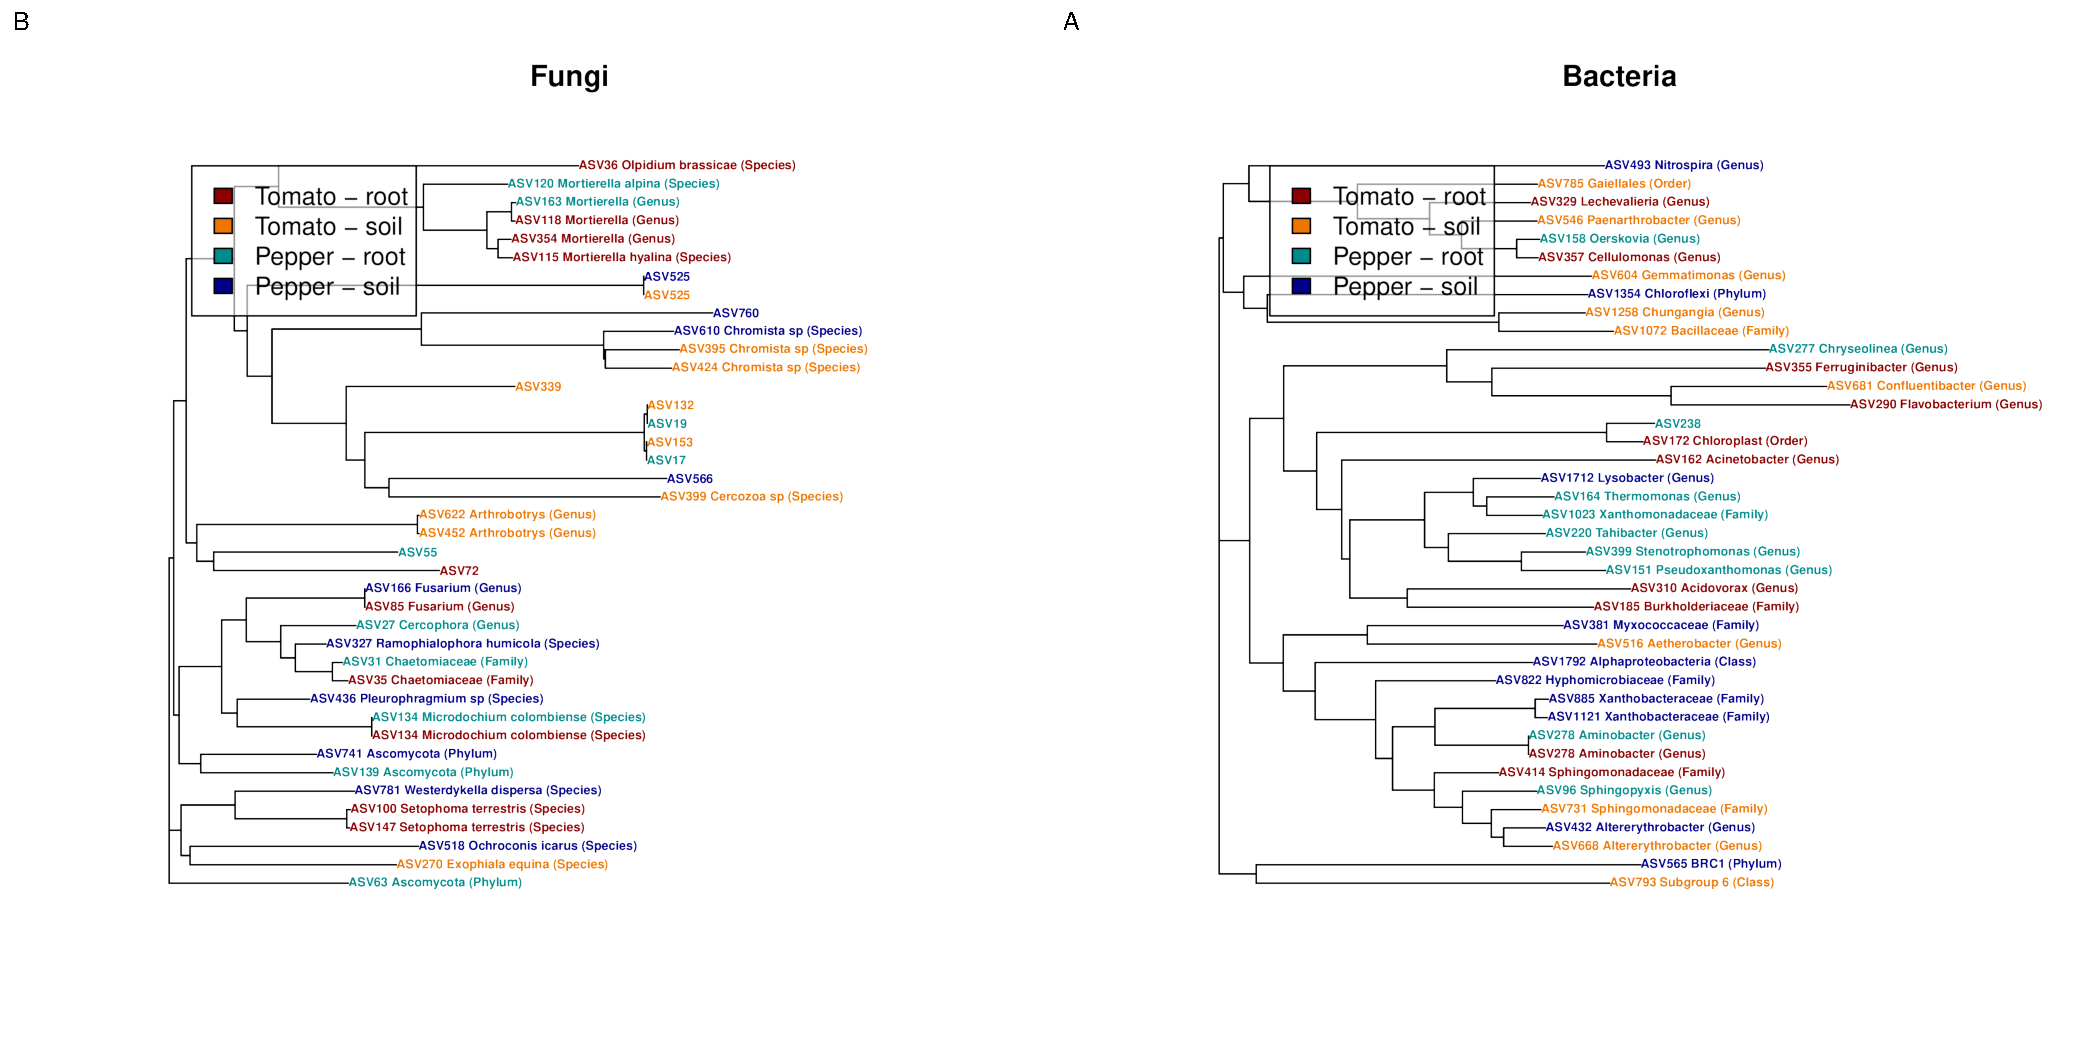
\includegraphics{../figures/Figure7_candidateASVs.pdf}\\
\textbf{Figure 7: Neighbor-Joining trees of candidates ASVs (fungi \&
roots) associated with productivity measures} ~\\
\hspace*{0.333em}

\newpage  

\section{DISCUSSION}\label{discussion}

\emph{• Brief recap of soil characteristics}\\
\emph{• Overall increases in productivity in both species (but mention
that tomato were fertilized with hen manure as well).} \emph{• Talk
about effect of treatment on root + soil diversity.}\\
\emph{• Talk about the fact in the roots, we most likely sequenced the
plant itself, rather than the bacteria.}\\
\emph{• Discuss some of the candidate ASVs from Figure 7.}

\newpage  

\section*{REFERENCES}\label{references}
\addcontentsline{toc}{section}{REFERENCES}

\hypertarget{refs}{}
\hypertarget{ref-altschul1997gapped}{}
Altschul SF., Madden TL., Schäffer AA., Zhang J., Zhang Z., Miller W.,
Lipman DJ. 1997. Gapped blast and psi-blast: A new generation of protein
database search programs. \emph{Nucleic acids research} 25:3389--3402.

\hypertarget{ref-anderson2001new}{}
Anderson MJ. 2001. A new method for non-parametric multivariate analysis
of variance. \emph{Austral ecology} 26:32--46.

\hypertarget{ref-anderson1999empirical}{}
Anderson MJ., Legendre P. 1999. An empirical comparison of permutation
methods for tests of partial regression coefficients in a linear model.
\emph{Journal of statistical computation and simulation} 62:271--303.

\hypertarget{ref-silva}{}
Callahan B. 2018. Silva for dada2: Silva taxonomic training data
formatted for dada2 (silva version 132). \emph{Zenodo}. DOI:
\href{https://doi.org/10.5281/zenodo.1172783}{10.5281/zenodo.1172783}.

\hypertarget{ref-callahan2016dada2}{}
Callahan BJ., McMurdie PJ., Rosen MJ., Han AW., Johnson AJA., Holmes SP.
2016. DADA2: High-resolution sample inference from illumina amplicon
data. \emph{Nature methods} 13:581.

\hypertarget{ref-caporaso2010qiime}{}
Caporaso JG., Kuczynski J., Stombaugh J., Bittinger K., Bushman FD.,
Costello EK., Fierer N., Pena AG., Goodrich JK., Gordon JI., others.
2010. QIIME allows analysis of high-throughput community sequencing
data. \emph{Nature methods} 7:335.

\hypertarget{ref-UNITE2017}{}
Community U. 2018.UNITE general fasta release. version 01.12.2017.
\emph{Available at}
\emph{\url{https://files.plutof.ut.ee/doi/C8/E4/C8E4A8E6A7C4C00EACE3499C51E550744A259A98F8FE25993B1C7B9E7D2170B2.zip}}

\hypertarget{ref-craigie2011seaweed}{}
Craigie JS. 2011. Seaweed extract stimuli in plant science and
agriculture. \emph{Journal of Applied Phycology} 23:371--393.

\hypertarget{ref-dumack2017rhogostomidae}{}
Dumack K., Flues S., Hermanns K., Bonkowski M. 2017. Rhogostomidae
(cercozoa) from soils, roots and plant leaves (arabidopsis thaliana):
Description of rhogostoma epiphylla sp. nov. and r. cylindrica sp. nov.
\emph{European journal of protistology} 60:76--86.

\hypertarget{ref-jukes1969evolution}{}
Jukes T., Cantor C. 1969. Evolution of protein molecules, pp. 21--132 in
mammalian protein metabolism, edited by munro hn.

\hypertarget{ref-klindworth2013evaluation}{}
Klindworth A., Pruesse E., Schweer T., Peplies J., Quast C., Horn M.,
Glöckner FO. 2013. Evaluation of general 16S ribosomal rna gene pcr
primers for classical and next-generation sequencing-based diversity
studies. \emph{Nucleic acids research} 41:e1--e1.

\hypertarget{ref-oksanen2013package}{}
Oksanen J., Blanchet FG., Kindt R., Legendre P., Minchin PR., O'hara R.,
Simpson GL., Solymos P., Stevens MHH., Wagner H., others. 2013. Package
``vegan''. \emph{Community ecology package, version} 2.

\hypertarget{ref-paradis2004ape}{}
Paradis E., Claude J., Strimmer K. 2004. APE: Analyses of phylogenetics
and evolution in r language. \emph{Bioinformatics} 20:289--290.

\hypertarget{ref-pinheiro2017nlme}{}
Pinheiro J., Bates D., DebRoy S., Sarkar D., Team RC. 2017. Nlme: Linear
and nonlinear mixedeffects models. r package version 3.1-128. 2016.
\emph{R software}.

\hypertarget{ref-schliep2010phangorn}{}
Schliep KP. 2010. Phangorn: Phylogenetic analysis in r.
\emph{Bioinformatics} 27:592--593.

\hypertarget{ref-schloss2009introducing}{}
Schloss PD., Westcott SL., Ryabin T., Hall JR., Hartmann M., Hollister
EB., Lesniewski RA., Oakley BB., Parks DH., Robinson CJ., others. 2009.
Introducing mothur: Open-source, platform-independent,
community-supported software for describing and comparing microbial
communities. \emph{Applied and environmental microbiology}
75:7537--7541.

\hypertarget{ref-toju2012high}{}
Toju H., Tanabe AS., Yamamoto S., Sato H. 2012. High-coverage its
primers for the dna-based identification of ascomycetes and
basidiomycetes in environmental samples. \emph{PloS one} 7:e40863.

\hypertarget{ref-wang2007naive}{}
Wang Q., Garrity GM., Tiedje JM., Cole JR. 2007. Naive bayesian
classifier for rapid assignment of rRNA sequences into the new bacterial
taxonomy. \emph{Applied and environmental microbiology} 73:5261--5267.

\hypertarget{ref-wickham2016ggplot2}{}
Wickham H. 2016. \emph{Ggplot2: Elegant graphics for data analysis}.
Springer.

\hypertarget{ref-wickham2015dplyr}{}
Wickham H., Francois R., Henry L., Müller K. 2015. Dplyr: A grammar of
data manipulation. \emph{R package version 0.4} 3.

\hypertarget{ref-wright2016using}{}
Wright ES. 2016. Using decipher v2. 0 to analyze big biological sequence
data in r. \emph{R Journal} 8.




\newpage
\singlespacing 
\end{document}
